\subsection{Benutzerschnittstelle}

\label{subsec:benutzerschnittstelle}

\begin{figure}[H]
	\centering
	\fbox{
		\begin{minipage}{13 cm}
			\centering
			\resizebox{100 mm}{!} {
				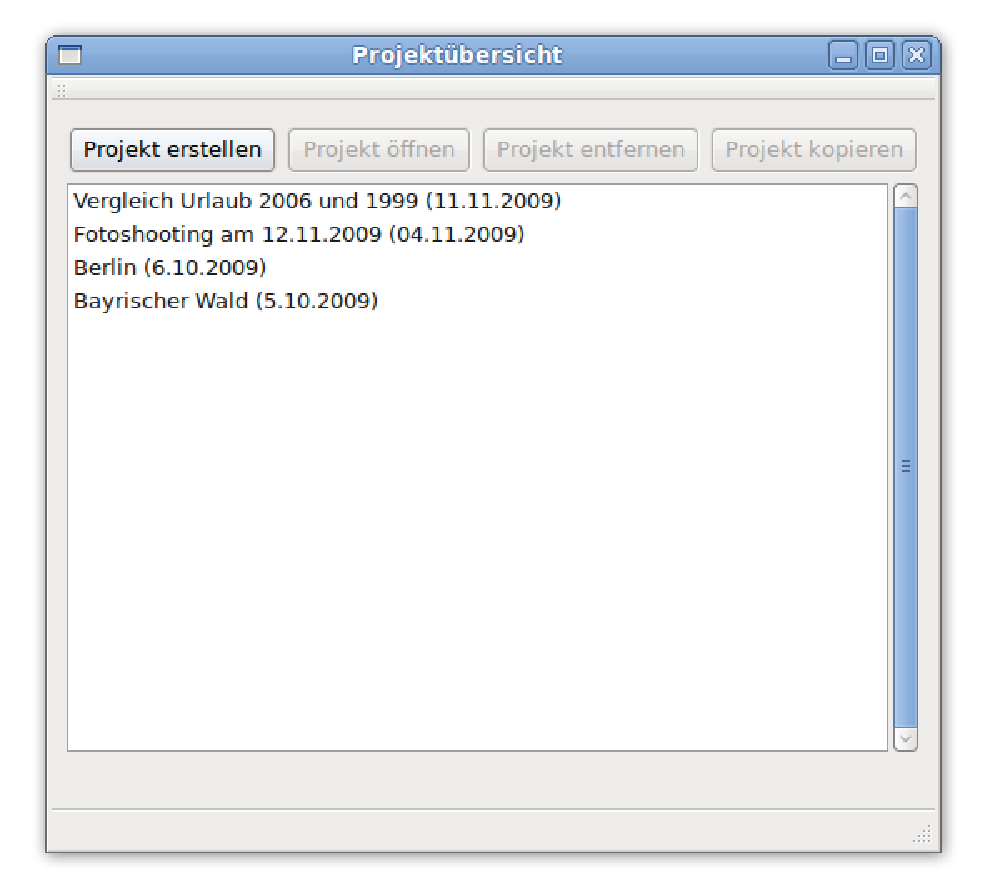
\includegraphics{images/mock-ups/projektverwaltung.eps}
			} 
			\caption{Die Projektübersicht}
			\label{gui:projektuebersicht}
		\end{minipage}  
	}    		
\end{figure} 


\begin{figure}[H]
	\centering
	\fbox{
		\begin{minipage}{13 cm}
			\centering
			\resizebox{113 mm}{!} {
				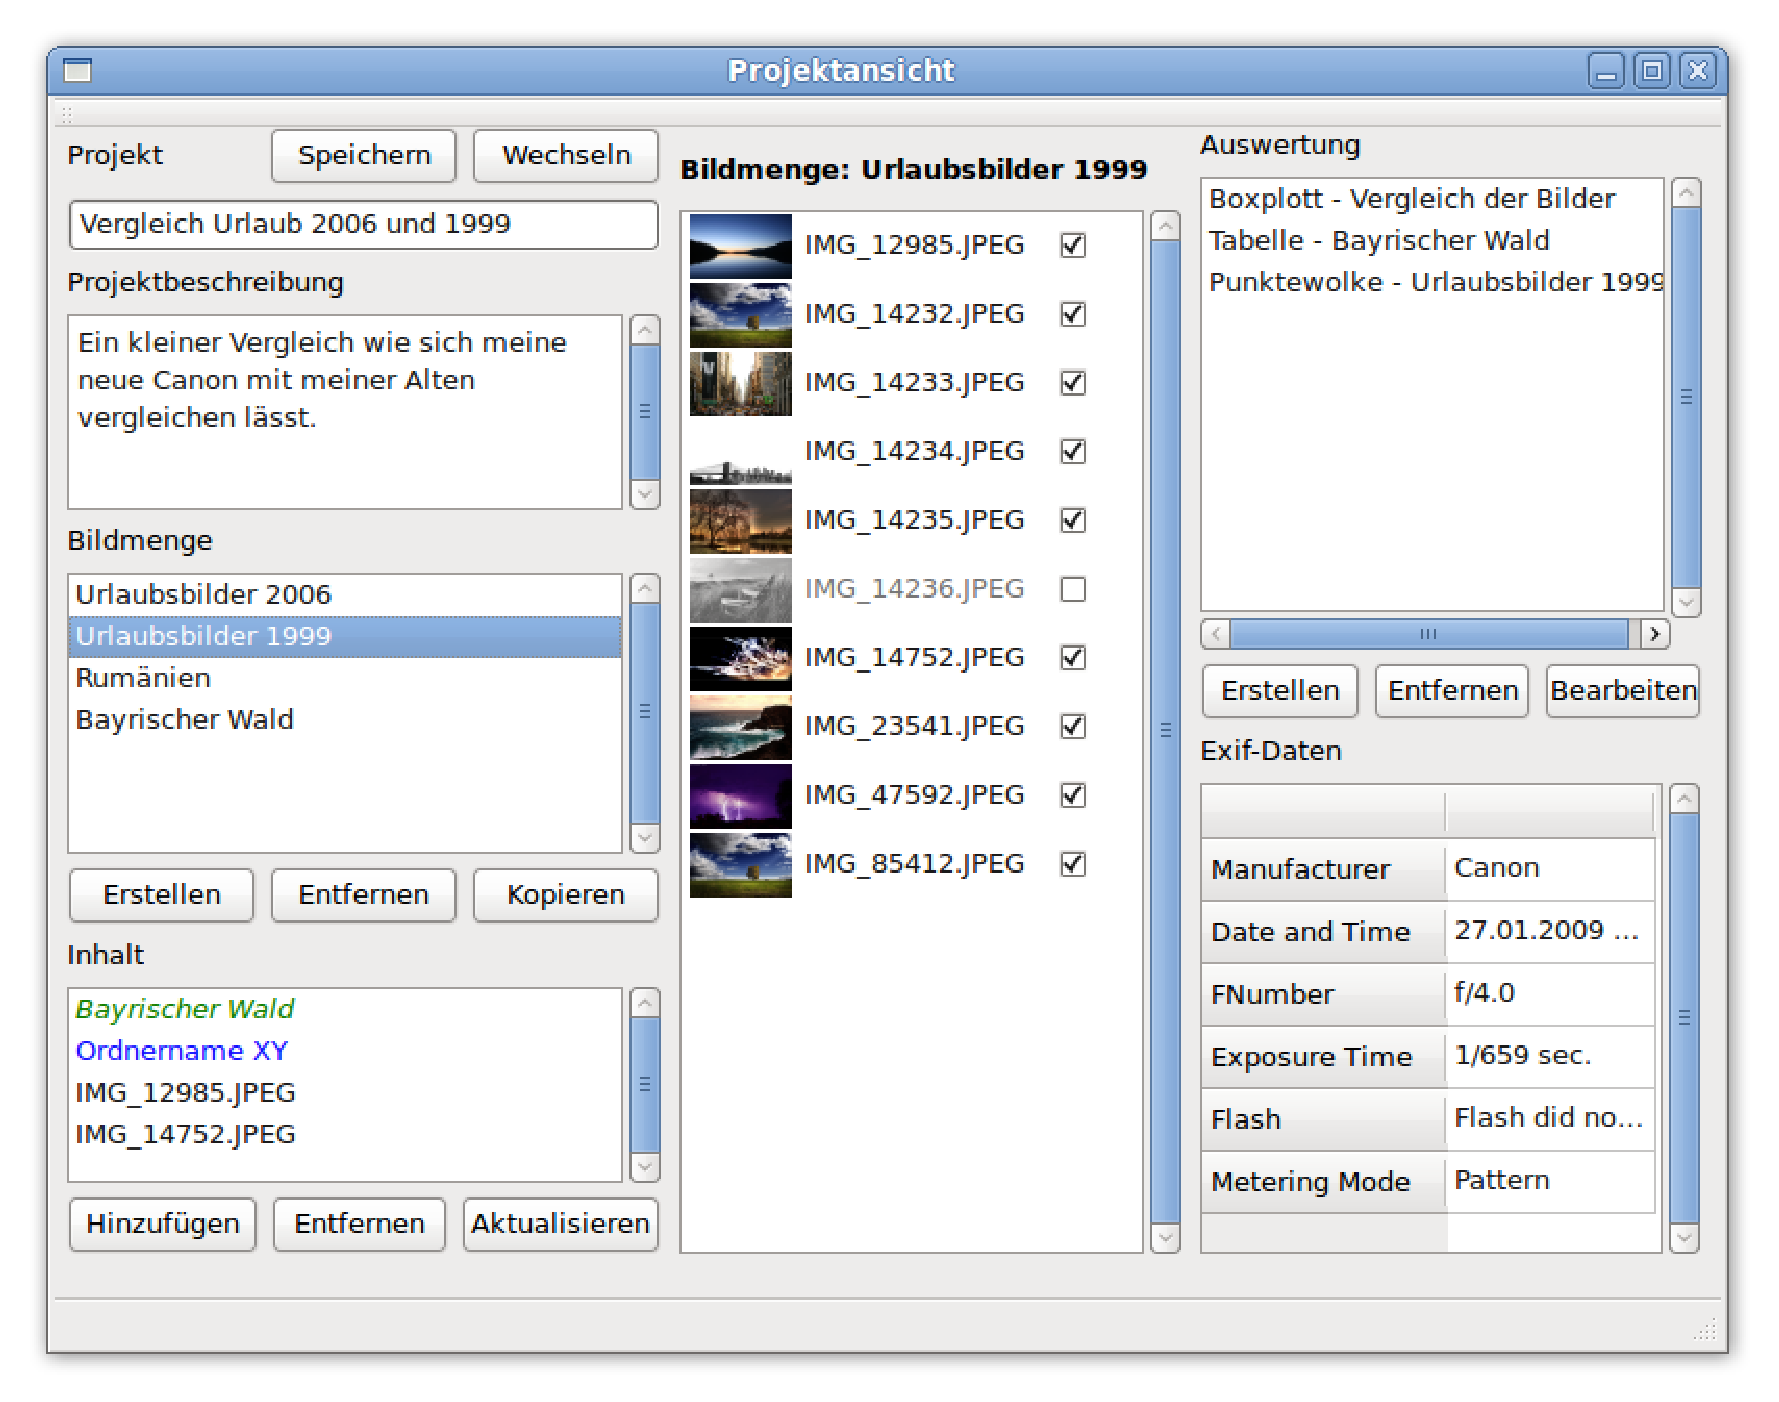
\includegraphics{images/mock-ups/projektansicht.eps}
			} 
			\caption{Die Projektansicht}
			\label{gui:projektansicht}
		\end{minipage}  
	}    		
\end{figure} 

\begin{figure}[H]
	\centering
	\fbox{
		\begin{minipage}{13 cm}
			\centering
			\resizebox{113 mm}{!} {
				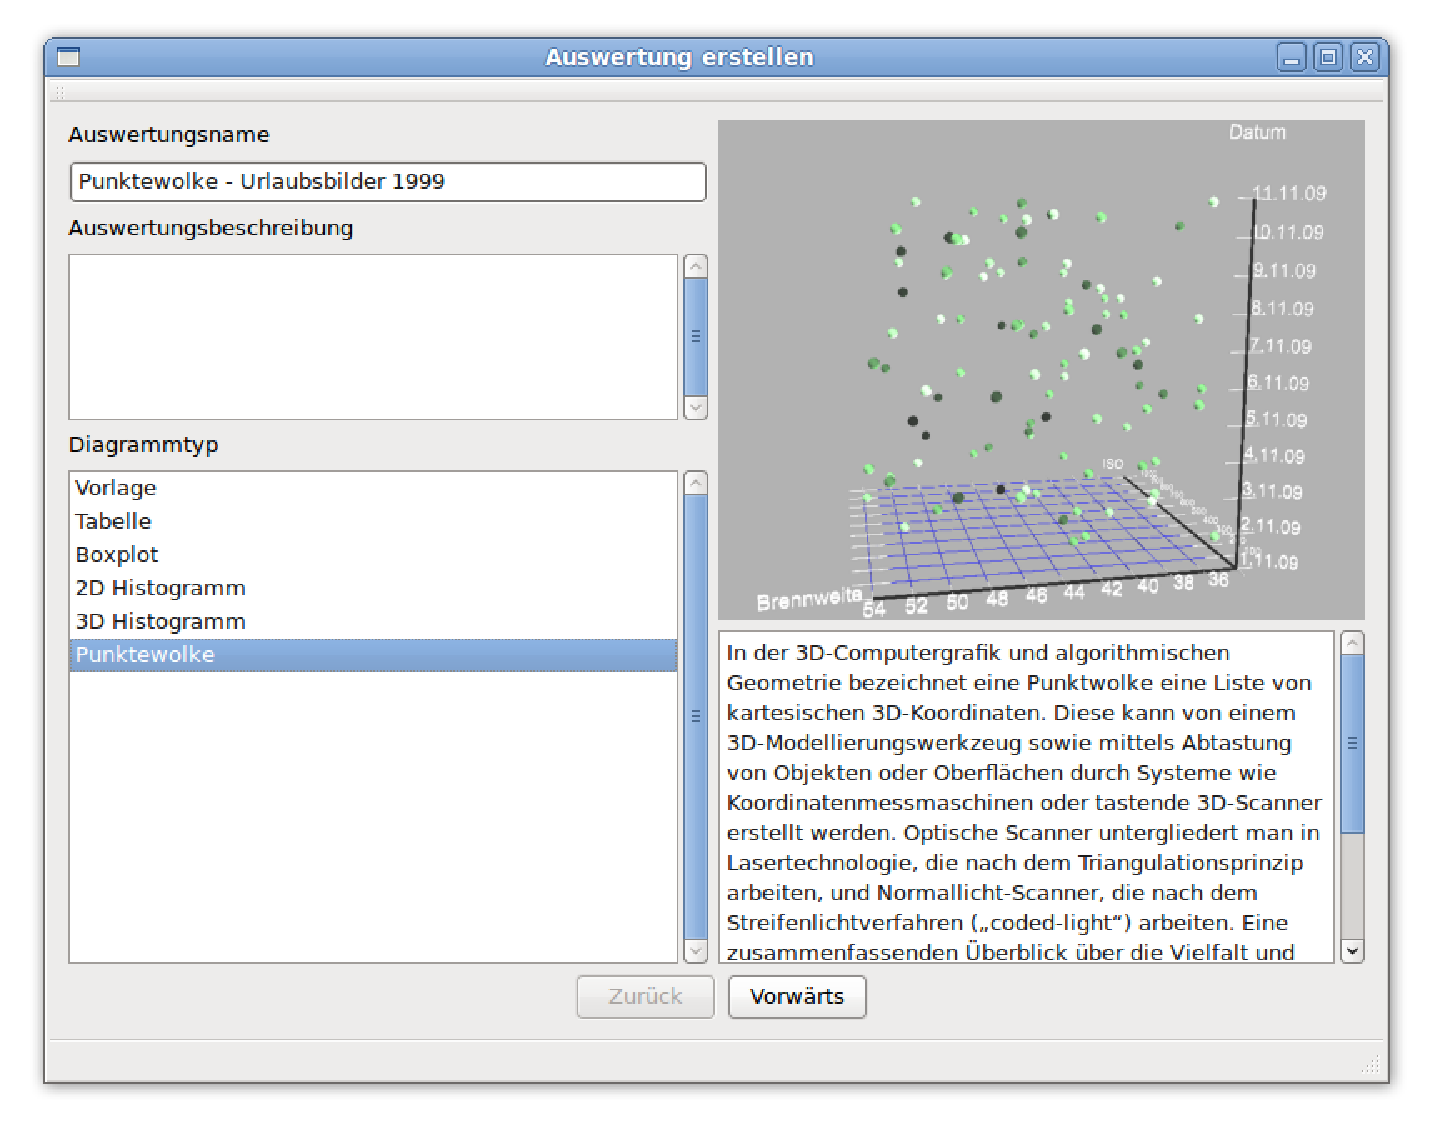
\includegraphics{images/mock-ups/auswertungseinstellungen.eps}
			} 
			\caption{Der Auswertungserstellungsassistent}
			\label{gui:auswertungseinstellungsassistent}
		\end{minipage}  
	}    		
\end{figure} 


\begin{figure}[H]
	\centering
	\fbox{
		\begin{minipage}{13 cm}
			\centering
			\resizebox{113 mm}{!} {
				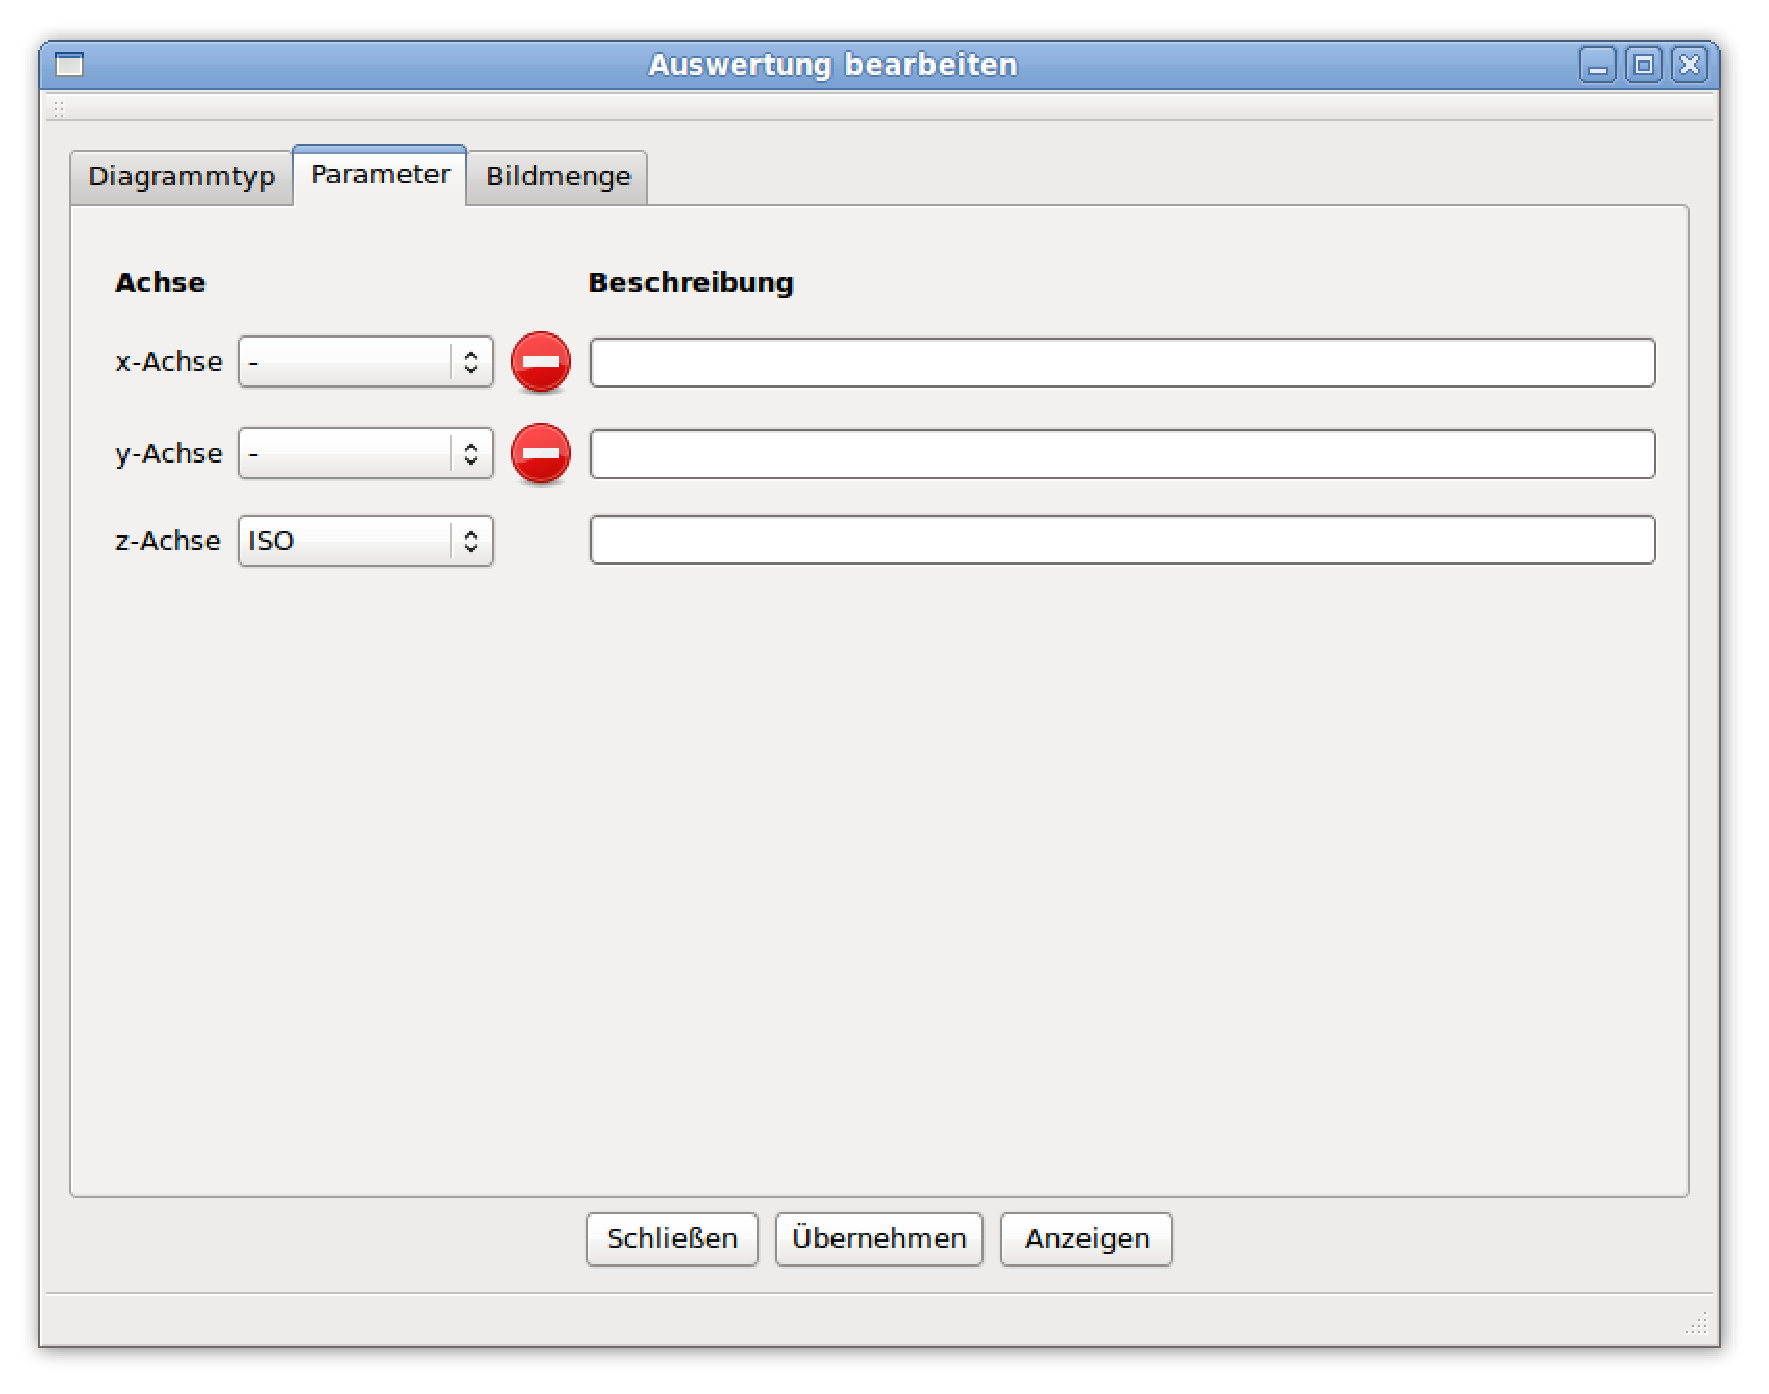
\includegraphics{images/mock-ups/parameter.eps}
			} 
			\caption{Die Parameterbearbeitung bei der Punktewolke}
			\label{gui:parameterbearbeitung}
		\end{minipage}  
	}    		
\end{figure} 

\begin{figure}[H]
	\centering
	\fbox{
		\begin{minipage}{13 cm}
			\centering
			\resizebox{113 mm}{!} {
				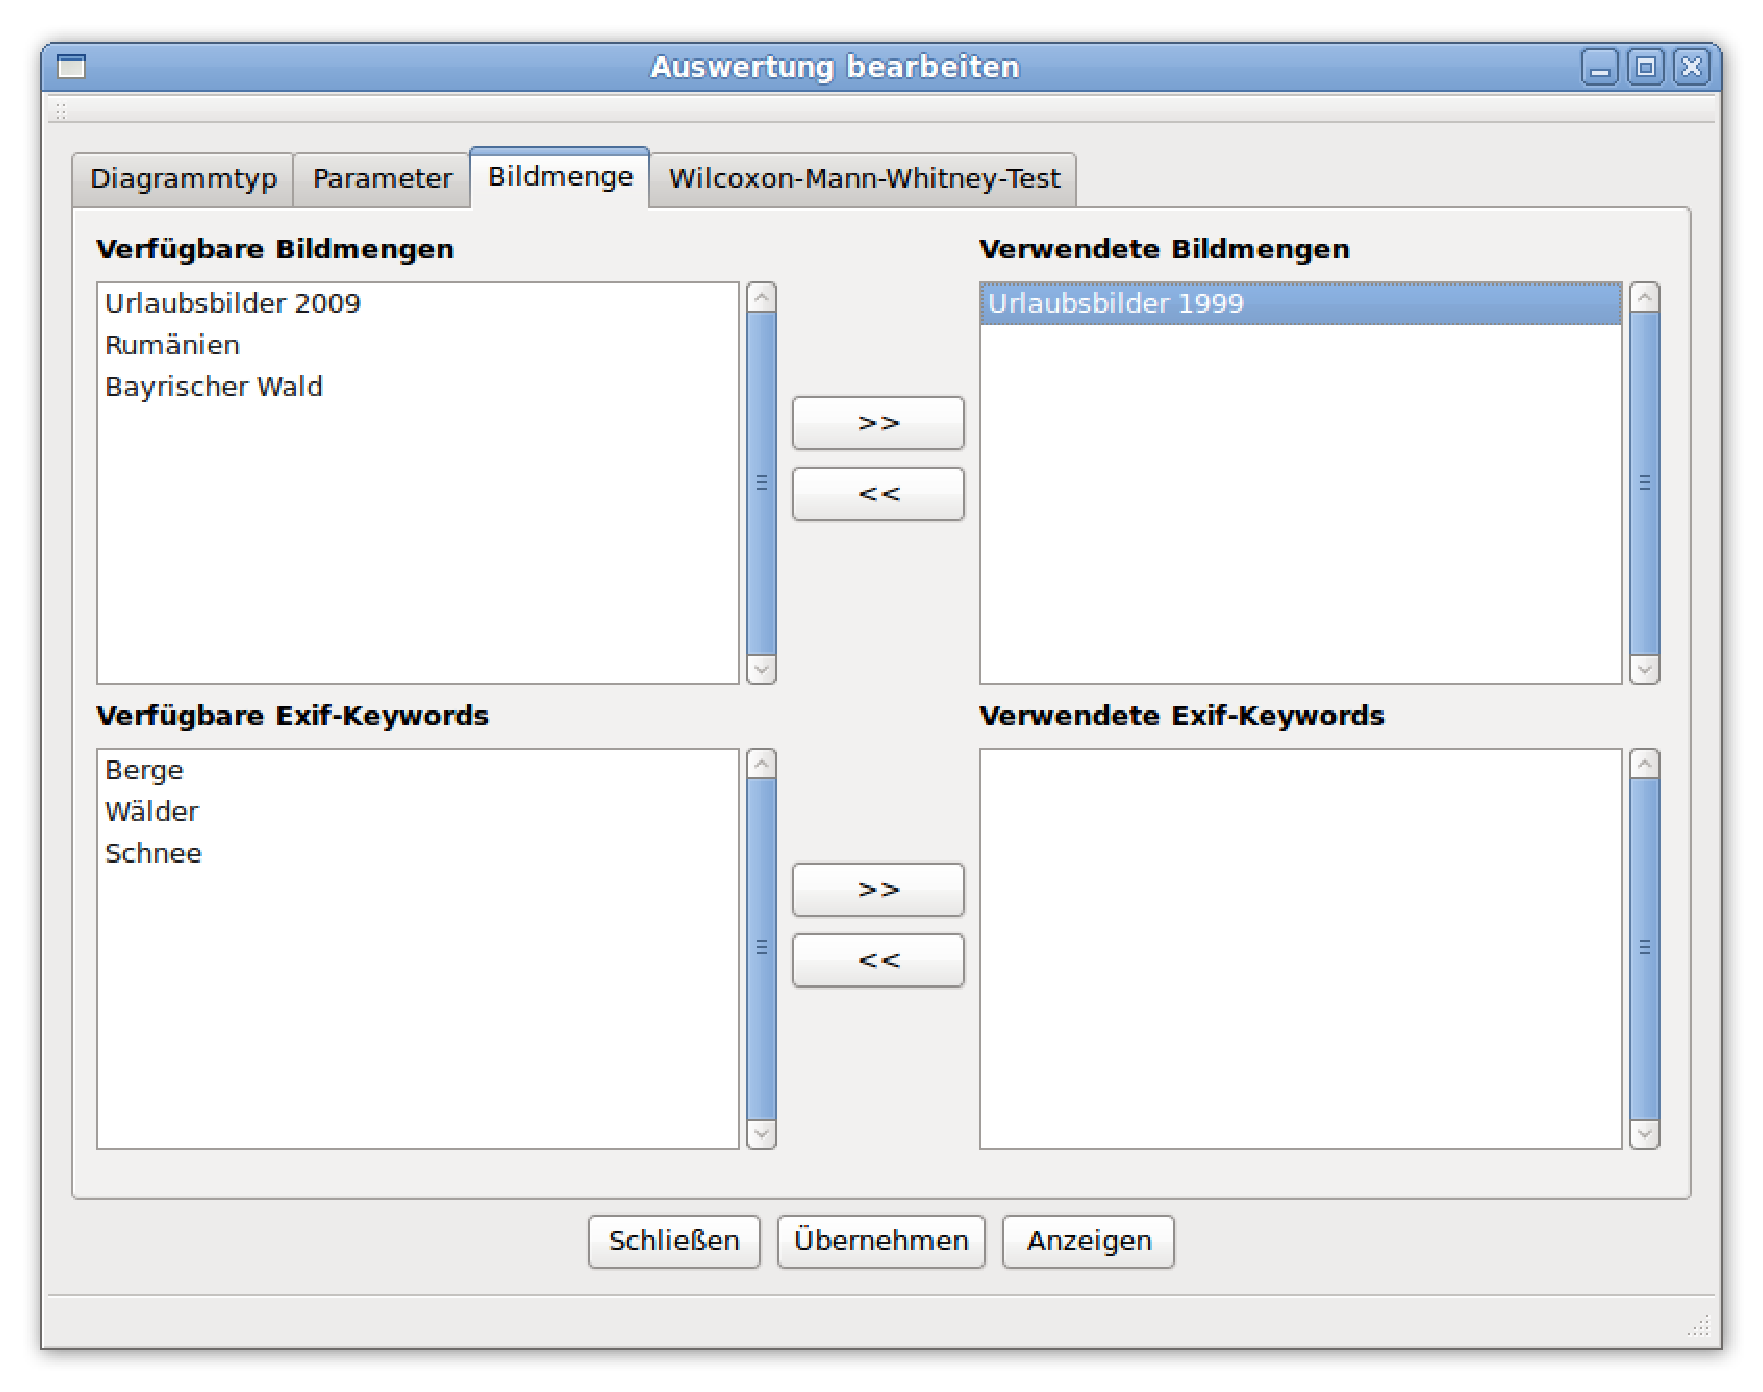
\includegraphics{images/mock-ups/bildmenge.eps}
			} 
			\caption{Die Bildmengenverwaltung innerhalb einer Auswertung}
			\label{gui:bildmengeverwalten}
		\end{minipage}  
	}    		
\end{figure} 

\begin{figure}[H]
	\centering
	\fbox{
		\begin{minipage}{13 cm}
			\centering
			\resizebox{113 mm}{!} {
				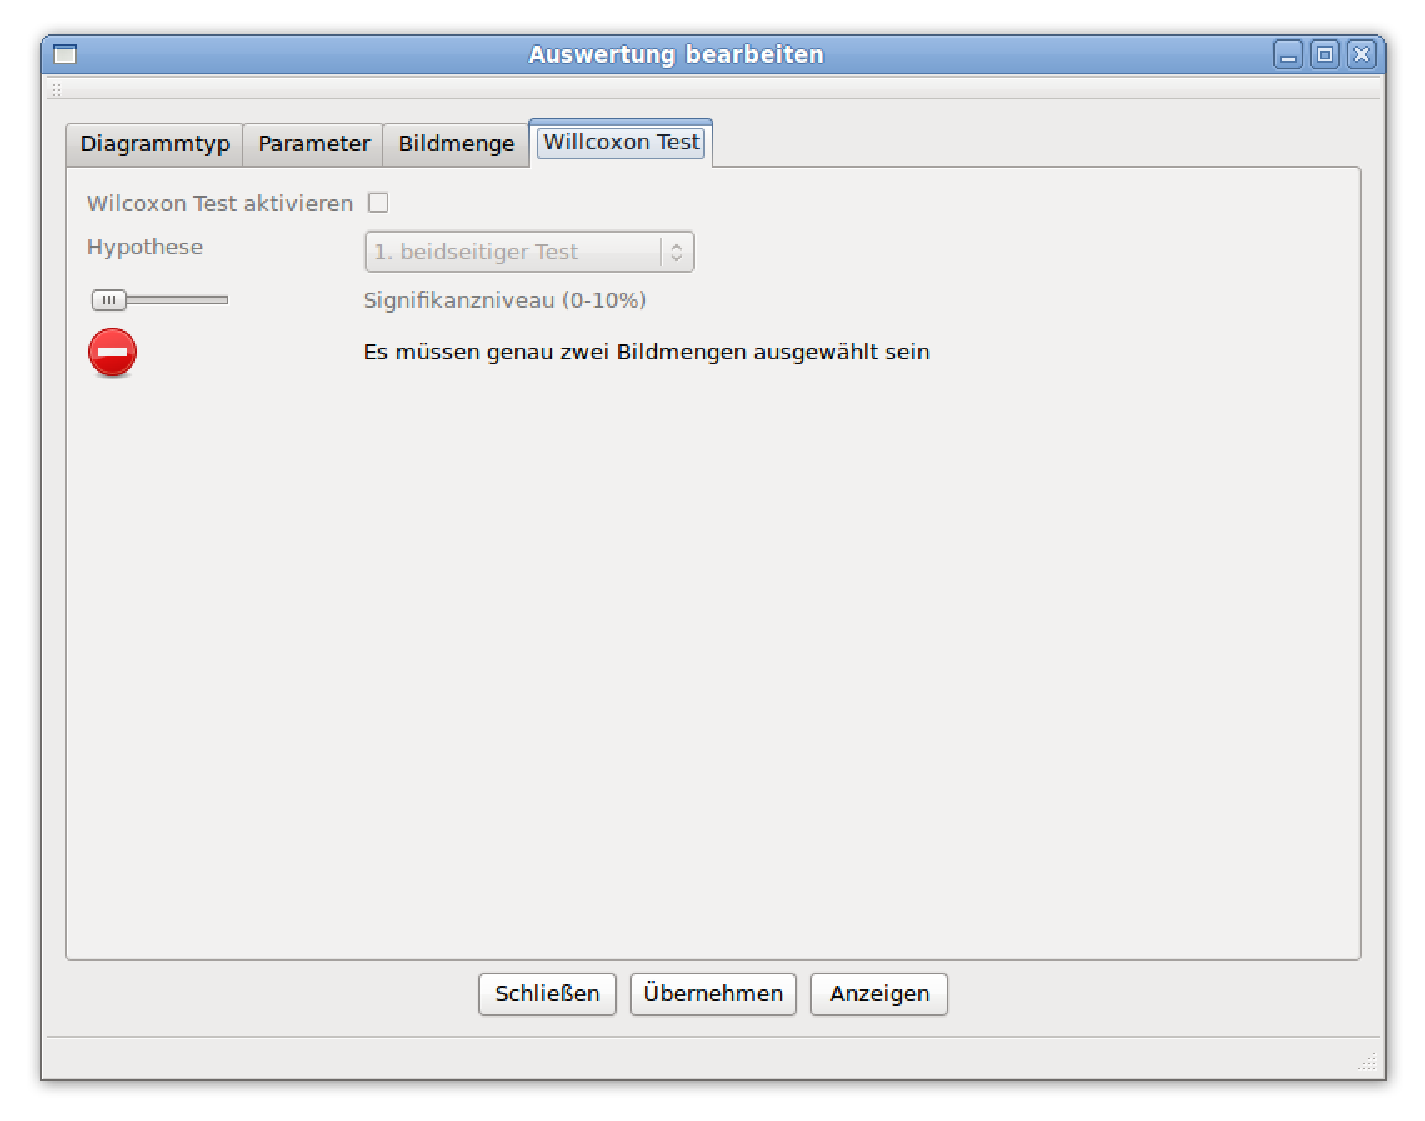
\includegraphics{images/mock-ups/willcoxon.eps}
			} 
			\caption{Der Wilcoxon-Mann-Whitney-Test innerhalb einer Boxplot Auswertung}
			\label{gui:willcoxon}
		\end{minipage}  
	}    		
\end{figure} 

\begin{figure}[H]
	\centering
	\fbox{
		\begin{minipage}{13 cm}
			\centering
			\resizebox{113 mm}{!} {
				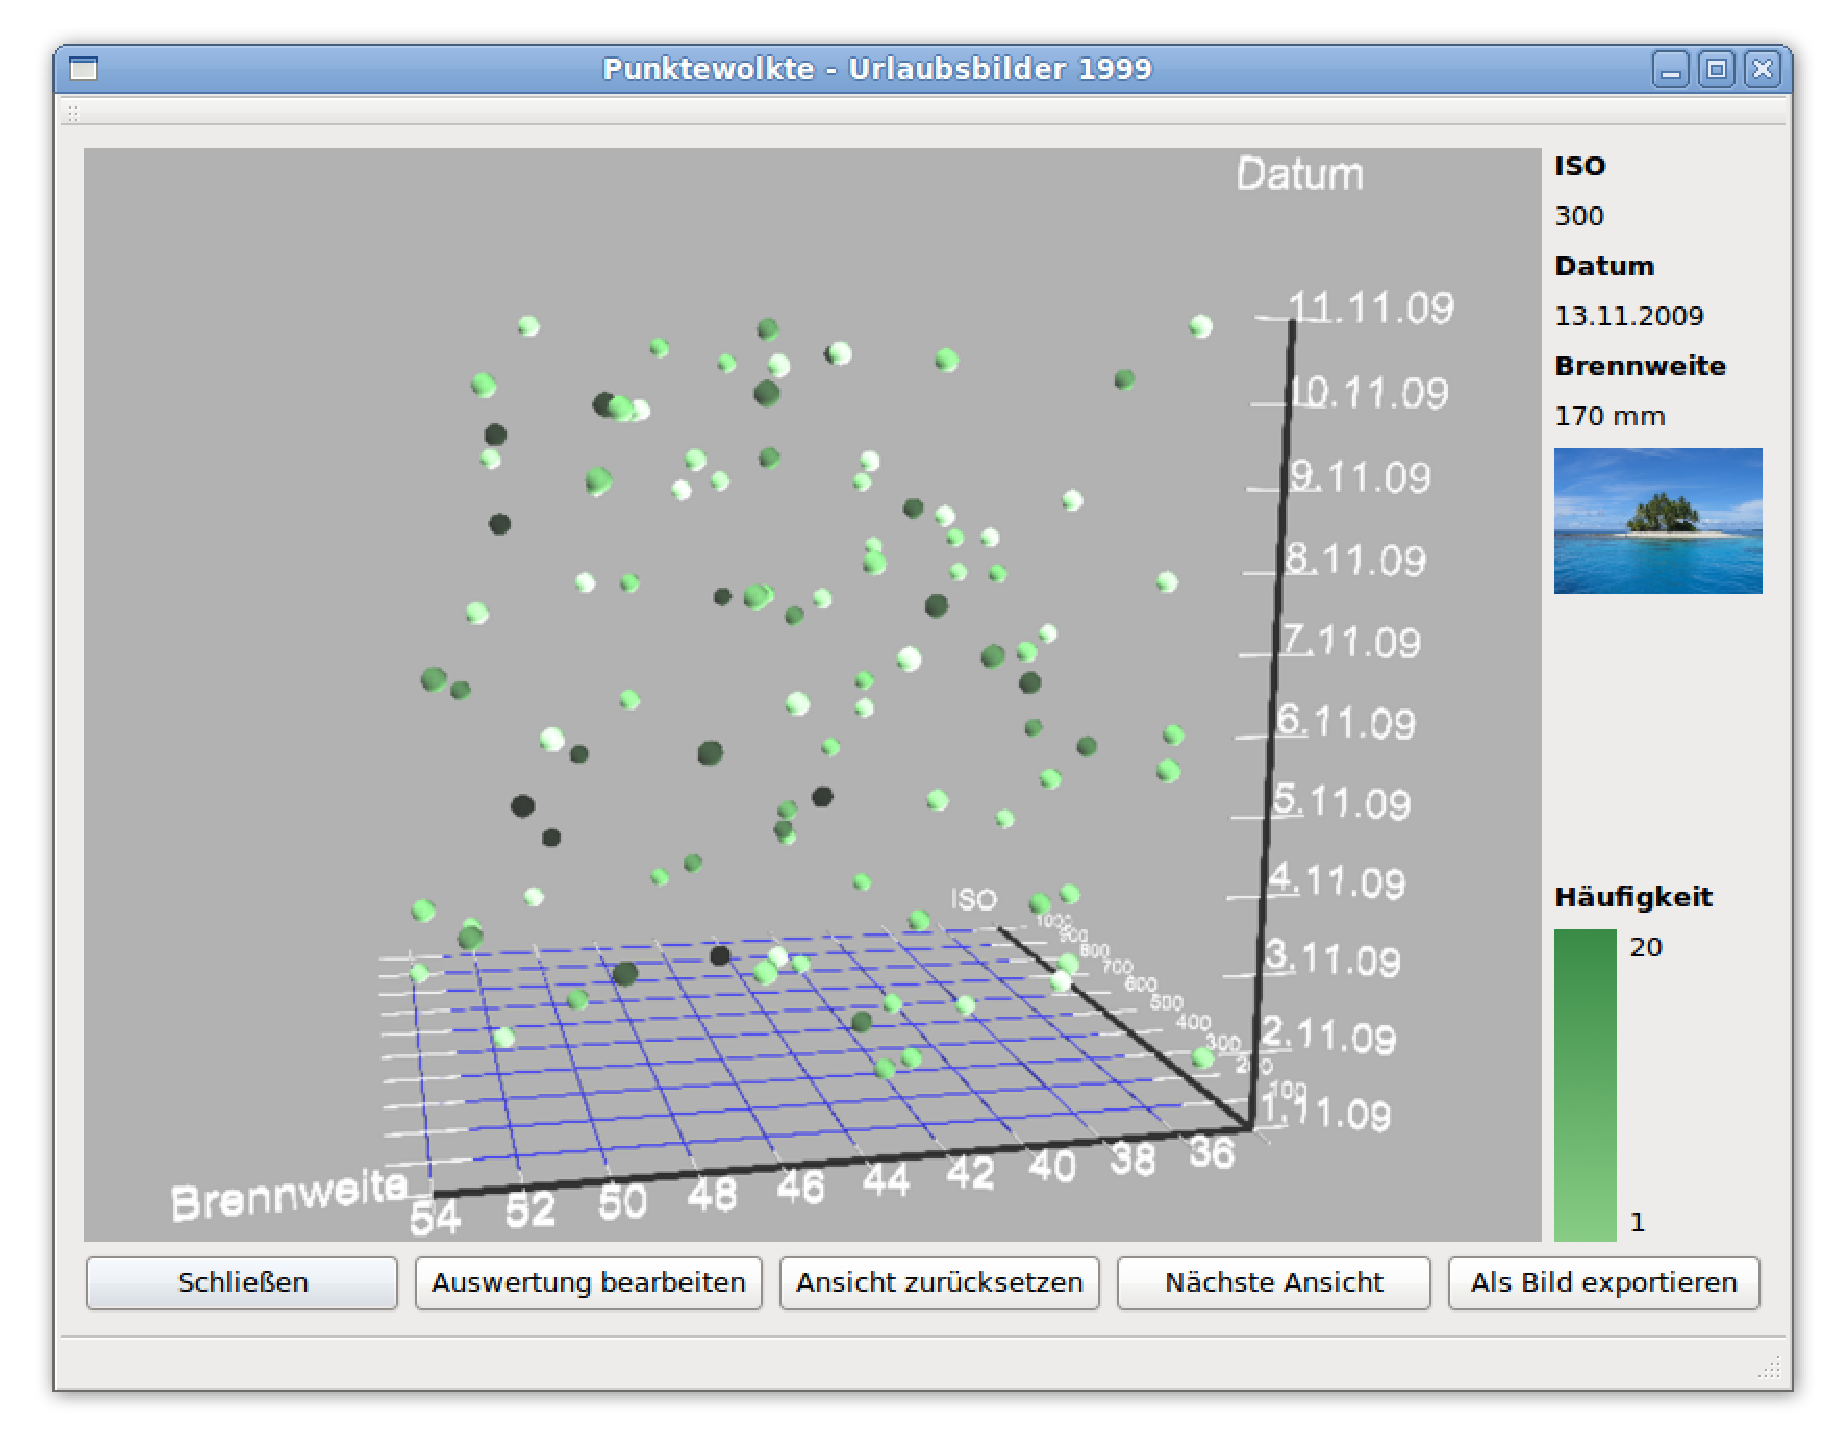
\includegraphics{images/mock-ups/ansichtpunktewolke.eps}
			} 
			\caption{Ansicht einer Auswertung mit Diagrammtyp Punktewolke}
			\label{gui:punktewolke}
		\end{minipage}  
	}    		
\end{figure} 